\documentclass{article}
\usepackage{tikz}
\usetikzlibrary{positioning}

\begin{document}

\begin{figure}[h]
    \centering
    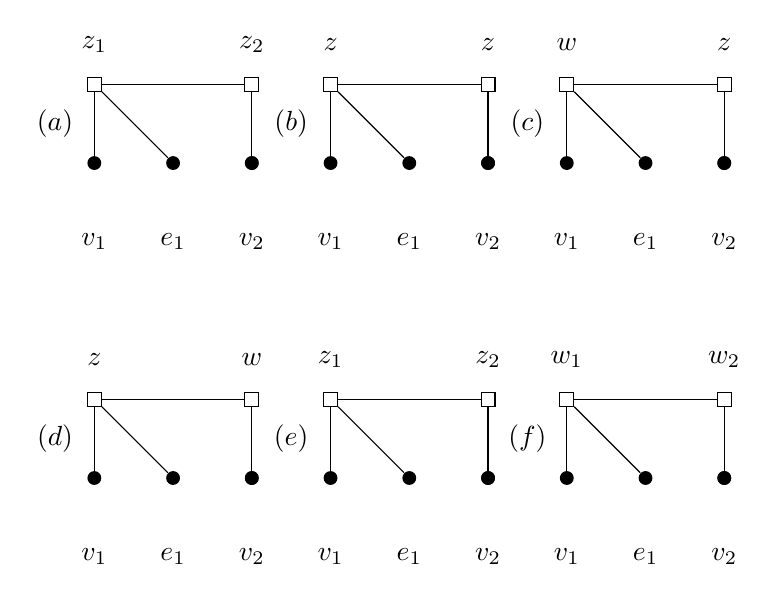
\begin{tikzpicture}[node distance=1cm, auto]
        % Define styles for nodes
        \tikzset{
            vertex/.style = {circle, fill, inner sep=0pt, minimum size=5pt},
            square/.style = {rectangle, draw, inner sep=0pt, minimum size=5pt},
        }

        % Node definitions
        \node[vertex] (v1) at (0, 0) {};
        \node[square] (z1) at (-1, 1) {};
        \node[vertex] (e1) at (-1, 0) {};
        \node[vertex] (v2) at (1, 0) {};
        \node[square] (z2) at (1, 1) {};
        \node[vertex] (e2) at (1, 0) {};

        % Draw edges
        \draw (v1) -- (z1);
        \draw (z1) -- (e1);
        \draw (z1) -- (z2);
        \draw (z2) -- (e2);
        \draw (z2) -- (v2);

        % Labels
        \node at (-1.5, 0.5) {$(a)$};
        \node at (-1, -1) {$v_1$};
        \node at (0, -1) {$e_1$};
        \node at (1, -1) {$v_2$};
        \node at (-1, 1.5) {$z_1$};
        \node at (1, 1.5) {$z_2$};

        % Repeat for other parts of the figure
        \begin{scope}[xshift=3cm]
            \node[vertex] (v1) at (0, 0) {};
            \node[square] (z1) at (-1, 1) {};
            \node[vertex] (e1) at (-1, 0) {};
            \node[vertex] (v2) at (1, 0) {};
            \node[square] (z2) at (1, 1) {};
            \node[vertex] (e2) at (1, 0) {};

            \draw (v1) -- (z1);
            \draw (z1) -- (e1);
            \draw (z1) -- (z2);
            \draw (z2) -- (e2);
            \draw (z2) -- (v2);

            \node at (-1.5, 0.5) {$(b)$};
            \node at (-1, -1) {$v_1$};
            \node at (0, -1) {$e_1$};
            \node at (1, -1) {$v_2$};
            \node at (-1, 1.5) {$z$};
            \node at (1, 1.5) {$z$};
        \end{scope}

        \begin{scope}[xshift=6cm]
            \node[vertex] (v1) at (0, 0) {};
            \node[square] (w) at (-1, 1) {};
            \node[vertex] (e1) at (-1, 0) {};
            \node[vertex] (v2) at (1, 0) {};
            \node[square] (z2) at (1, 1) {};
            \node[vertex] (e2) at (1, 0) {};

            \draw (v1) -- (w);
            \draw (w) -- (e1);
            \draw (w) -- (z2);
            \draw (z2) -- (e2);
            \draw (z2) -- (v2);

            \node at (-1.5, 0.5) {$(c)$};
            \node at (-1, -1) {$v_1$};
            \node at (0, -1) {$e_1$};
            \node at (1, -1) {$v_2$};
            \node at (-1, 1.5) {$w$};
            \node at (1, 1.5) {$z$};
        \end{scope}

        \begin{scope}[yshift=-4cm]
            \node[vertex] (v1) at (0, 0) {};
            \node[square] (z) at (-1, 1) {};
            \node[vertex] (e1) at (-1, 0) {};
            \node[vertex] (v2) at (1, 0) {};
            \node[square] (w) at (1, 1) {};
            \node[vertex] (e2) at (1, 0) {};

            \draw (v1) -- (z);
            \draw (z) -- (e1);
            \draw (z) -- (w);
            \draw (w) -- (e2);
            \draw (w) -- (v2);

            \node at (-1.5, 0.5) {$(d)$};
            \node at (-1, -1) {$v_1$};
            \node at (0, -1) {$e_1$};
            \node at (1, -1) {$v_2$};
            \node at (-1, 1.5) {$z$};
            \node at (1, 1.5) {$w$};
        \end{scope}

        \begin{scope}[xshift=3cm, yshift=-4cm]
            \node[vertex] (v1) at (0, 0) {};
            \node[square] (z1) at (-1, 1) {};
            \node[vertex] (e1) at (-1, 0) {};
            \node[vertex] (v2) at (1, 0) {};
            \node[square] (z2) at (1, 1) {};
            \node[vertex] (e2) at (1, 0) {};

            \draw (v1) -- (z1);
            \draw (z1) -- (e1);
            \draw (z1) -- (z2);
            \draw (z2) -- (e2);
            \draw (z2) -- (v2);

            \node at (-1.5, 0.5) {$(e)$};
            \node at (-1, -1) {$v_1$};
            \node at (0, -1) {$e_1$};
            \node at (1, -1) {$v_2$};
            \node at (-1, 1.5) {$z_1$};
            \node at (1, 1.5) {$z_2$};
        \end{scope}

        \begin{scope}[xshift=6cm, yshift=-4cm]
            \node[vertex] (v1) at (0, 0) {};
            \node[square] (w1) at (-1, 1) {};
            \node[vertex] (e1) at (-1, 0) {};
            \node[vertex] (v2) at (1, 0) {};
            \node[square] (w2) at (1, 1) {};
            \node[vertex] (e2) at (1, 0) {};

            \draw (v1) -- (w1);
            \draw (w1) -- (e1);
            \draw (w1) -- (w2);
            \draw (w2) -- (e2);
            \draw (w2) -- (v2);

            \node at (-1.5, 0.5) {$(f)$};
            \node at (-1, -1) {$v_1$};
            \node at (0, -1) {$e_1$};
            \node at (1, -1) {$v_2$};
            \node at (-1, 1.5) {$w_1$};
            \node at (1, 1.5) {$w_2$};
        \end{scope}
    \end{tikzpicture}
\end{figure}

\end{document}